\documentclass[11pt,a4paper]{article}

\usepackage[utf8]{inputenc}
\usepackage[T1]{fontenc}
\usepackage[english]{babel}
\usepackage{geometry}
\geometry{top=2.5cm, bottom=2.5cm, left=2.5cm, right=2.5cm}
\usepackage{fancyhdr}
\usepackage{lastpage}
\usepackage{booktabs}
\usepackage{tabularx}
\usepackage{longtable}
\usepackage{float}
\usepackage{graphicx}
\usepackage{xcolor}
\usepackage{hyperref}
\usepackage{listings}
\usepackage{enumitem}
\usepackage{amsmath,amssymb}
\usepackage{microtype}

\definecolor{navyblue}{RGB}{20, 50, 90}
\definecolor{codebg}{RGB}{248, 249, 250}

\hypersetup{
    pageanchor=false,
    colorlinks=true,
    linkcolor=navyblue,
    urlcolor=navyblue,
    citecolor=navyblue
}

\pagestyle{fancy}
\fancyhf{}
\fancyhead[L]{\small WellProdSim / EthosTerra}
\fancyhead[R]{\small Progress Report -- Week 11 (Block B7: Decoupled Integration)}
\fancyfoot[C]{\small \thepage\ of \pageref{LastPage}}
\renewcommand{\headrulewidth}{0.4pt}
\renewcommand{\footrulewidth}{0pt}

\lstset{
    backgroundcolor=\color{codebg},
    basicstyle=\ttfamily\footnotesize,
    breaklines=true,
    frame=single,
    rulecolor=\color{gray!30},
    numbers=none,
    showstringspaces=false
}

\begin{document}

% ==============================================================================
% TITLE PAGE
% ==============================================================================
\begin{titlepage}
    \thispagestyle{empty}
    \centering
    \vspace*{1.5cm}

    {\large Universidad Tecnol\'ogica de Bol\'ivar\par}
    \vspace{0.3cm}
    {\normalsize Master of Science in Engineering -- Research Seminar II\par}

    \vspace{2.0cm}
    {\LARGE\bfseries Decoupled Integration with EthosTerra, Synthesis of Institutional Equations with Formal Verification, and Veracity Validation\par}

    \vspace{0.8cm}
    {\large\itshape Progress Report -- Week 11 of 16\par}

    \vspace{2.2cm}
    \begin{tabular}{ll}
        \textbf{Researcher:} & Jes\'us Mart\'inez Velandia \\
        \textbf{Advisor:} & Jairo Serrano \\
        \textbf{Co-advisors:} & Edwin Puertas, Juan Mart\'inez \\
        \textbf{Period:} & Week 11 of 16 \\
        \textbf{Block:} & B7: Decoupled Integration and Macro--Micro Mapping \\
        \textbf{Date:} & October 22, 2026 \\
    \end{tabular}

    \vfill
    {\small Consolidated technical version backed by empirical, graphical, and mathematical evidence\par}
    \vspace*{1.0cm}
\end{titlepage}

\clearpage
\hypersetup{pageanchor=true}
\pagenumbering{roman}
\setcounter{page}{1}
\fancyfoot[C]{\small \thepage}
\tableofcontents
\clearpage

% ==============================================================================
% 1. OPERATIONAL SCOPE AND CONTEXT
% ==============================================================================
\pagenumbering{arabic}
\setcounter{page}{1}
\fancyfoot[C]{\small \thepage\ of \pageref{LastPage}}

\section{Operational scope of Week 11 in the project roadmap}

Week 11 establishes the operational transition between the territorial eBDI Atlas (Block B6) and preparatory groundwork for multi-agent simulation coupling with WellProdSim / Python BESA (Blocks B7 through B9). During this phase, the project addresses the ontological and semantic alignment between public agrarian policies and the micro-agronomic behavioral dynamics of peasant agents.

\begin{table}[H]
\centering
\small
\caption{Roadmap and evolutionary milestone status of the research project.}
\label{tab:roadmap}
\begin{tabularx}{\textwidth}{lp{3.2cm}p{5.2cm}X}
\toprule
\textbf{Week} & \textbf{Block} & \textbf{Milestone Goal} & \textbf{Status} \\
\midrule
Week 5 & B1 (Baseline) & Canary classifier across 20 DMR scenarios & Completed (\texttt{388553e}) \\
Week 6 & B2--B3 (Pure Case) & Pydantic V2 contracts and EvidenceSpan & Completed (\texttt{30090dc}) \\
Week 7 & B4 (Conflict Case) & Physical collision detection in 30 scenarios & Completed (\texttt{b3f810a}) \\
Week 8 & B5 (Manual CRUD) & Decoupled persistence and retained trash & Completed (\texttt{a140f22}) \\
Week 9 & B6 (Atlas and Corpus) & Atlas AT-1, SHA-256 quarantine, YAML compiler & Completed (\texttt{d17e44b}) \\
Week 10 & Deployment and Security & Dokploy cloud production, Zero-Trust, JWT auth & Completed (\texttt{e477f57}) \\
\textbf{Week 11} & \textbf{B7 (BESA Integration)} & \textbf{Decoupled adapter, AST oracle, equations} & \textbf{Completed (\texttt{HEAD})} \\
Week 12 & B8--B9 (BDI Sandbox) & Deliberation, equilibrium, multi-agent tests & Scheduled \\
\bottomrule
\end{tabularx}
\end{table}

% ==============================================================================
% 2. ONTOLOGICAL GAP AND THREE-TIER ARCHITECTURE
% ==============================================================================
\section{Ontological gap diagnosis and three-tier knowledge model}

In early development stages, the information extraction subsystem treated all documentary inputs indistinctly as direct individual beliefs and personal intentions of peasant agents. This created ontological contradictions: real peasant families in Montes de Mar\'ia do not deliberate upon international treaty quotas or ministerial budgetary allocations; their daily decision space is constrained by a 24-hour labor budget, a \$12,000 COP basic daily survival threshold, bank debt obligations, and localized water availability on their parcels.

To resolve this ontological dissonance, the architectural design of this research decomposes territorial knowledge into three disjoint, stratified levels, grounding classical Belief-Desire-Intention deliberative agent theory (Bratman, 1987; Rao and Georgeff, 1995), the Ortony-Clore-Collins affective dynamics model (Ortony, Clore, and Collins, 1988), and institutional common-pool resource governance theory (Ostrom, 1990):

\begin{enumerate}[leftmargin=*]
    \item \textbf{Peasant Narratives and Daily Logs (Micro Level):} Encode internal eBDI psychological states, OCC emotional balance (Joy, Distress, Hope, Fear), physiological thresholds, and daily vital trade-offs. These compile directly into executable \texttt{GoalSpec} and \texttt{PlanSpec} structures.
    \item \textbf{Land-Use Territorial Plans (POT/PBOT) (Meso-Physical Level):} Define spatial topology, transport connectivity graphs, and hard biophysical boundaries (such as impassable river buffer zones with $\text{isWalkable} = \text{false}$, and Family Agricultural Units UAF defined by DANE, 2024).
    \item \textbf{Agrarian Public Policies and Laws (Macro-Institutional Level):} Do not constitute individual peasant desires; they define the institutional rules of the game, structural economic incentives, and operational functions governing environmental simulation entities in EthosTerra (Ostrom, 1990): \texttt{BankOffice} (lending interest rate curves), \texttt{MarketPlace} (support pricing floors under Law 2046 of 2020), \texttt{CivicAuthority} (input subsidies), and \texttt{AgroEcosystem} (irrigation district quotas following Allen et al., 1998). These compile into the newly specified \texttt{InstitutionalPolicySpec} contract.
\end{enumerate}

% ==============================================================================
% 3. AGENT RULES, EXTRACTION AND FORMAL VERACITY VALIDATION PROTOCOL
% ==============================================================================
\section{Micro-LLM agent prompt rules, symbolic extraction, and formal veracity validation}

A core contribution of Block B7 is the formalization of how the extraction agent synthesizes parametric equations and, crucially, \textbf{how their mathematical and normative veracity is rigorously validated} against empirical sources, preventing both hallucination and unconstrained code execution.

\subsection{Micro-LLM agent role and governed inference prompt rules}

The project's designated micro-LLM model is \texttt{ai/gemma4:E4B}, executed offline-first via Docker Model Runner (DMR) to preserve strict data sovereignty. To ensure deterministic convergence and factual truthfulness, the agent operates under rigid prompt engineering boundaries:

\begin{itemize}[leftmargin=*]
    \item \textbf{Context Isolation and Delimitation:} Source texts are injected strictly inside delimited \texttt{<document\_context>} tags, fully segregating data from instruction channels to eliminate prompt injection risks.
    \item \textbf{Rigid Pydantic V2 Schema (\texttt{extra="forbid"}):} The micro-LLM output is strictly validated against a rigid JSON schema defining \texttt{ParametricEquationSpec}. Any unexpected or unrecognized field causes instantaneous rejection at the deserialization stage.
    \item \textbf{Pure Symbolic Syntax Restriction:} The model is strictly prohibited from emitting free Python code, control loops (\texttt{for}, \texttt{while}), conditional branches (\texttt{if}), or anonymous functions (\texttt{lambda}). The agent may only propose pure analytic mathematical expressions (e.g., \texttt{base * (1 - delta * s)}).
    \item \textbf{Explicit Boundary and Behavioral Declarations:} The prompt requires the LLM to explicitly declare input domain limits $[x_{\min}, x_{\max}]$, admissible output range $[y_{\min}, y_{\max}]$, the target simulation entity, and expected monotonicity behavior (\texttt{increasing}, \texttt{decreasing}, \texttt{constant}).
\end{itemize}

\subsection{Extraction mechanics and decoupled simulation pipeline}

The extraction and deployment lifecycle operates through a four-stage pipeline:
\begin{enumerate}[leftmargin=*]
    \item \textbf{Document Ingestion and Quarantine:} Authoritative legal and technical documents (e.g., Law 2046 of 2020, PATR Montes de Mar\'ia ART 2019) reside in the document quarantine store (\texttt{data/quarantine/}) under immutable SHA-256 cryptographic hashes.
    \item \textbf{Textual Segmentation:} Documents are partitioned into contextual windows preserving page references and byte offsets (\texttt{EvidenceSpan}).
    \item \textbf{Parametric Extraction:} The micro-LLM analyzes the segment and outputs the structured \texttt{ParametricEquationSpec} candidate.
    \item \textbf{Decoupled Compilation:} \texttt{EBDIYamlCompiler} serializes the policy into \texttt{outputs/atlas/yaml/institutional/}. Subsequently, the \texttt{EthosTerraDecoupledAdapter} transforms these specifications into operational modifiers in \texttt{outputs/simulation\_sandbox/world\_modifiers.json}, without altering a single line of the core \texttt{EthosTerra} repository.
\end{enumerate}

\subsection{Four-layer veracity validation protocol}

To guarantee that generated equations do not represent stochastic hallucinations, the architecture implements a multi-tier deterministic verification battery:

\begin{figure}[H]
    \centering
    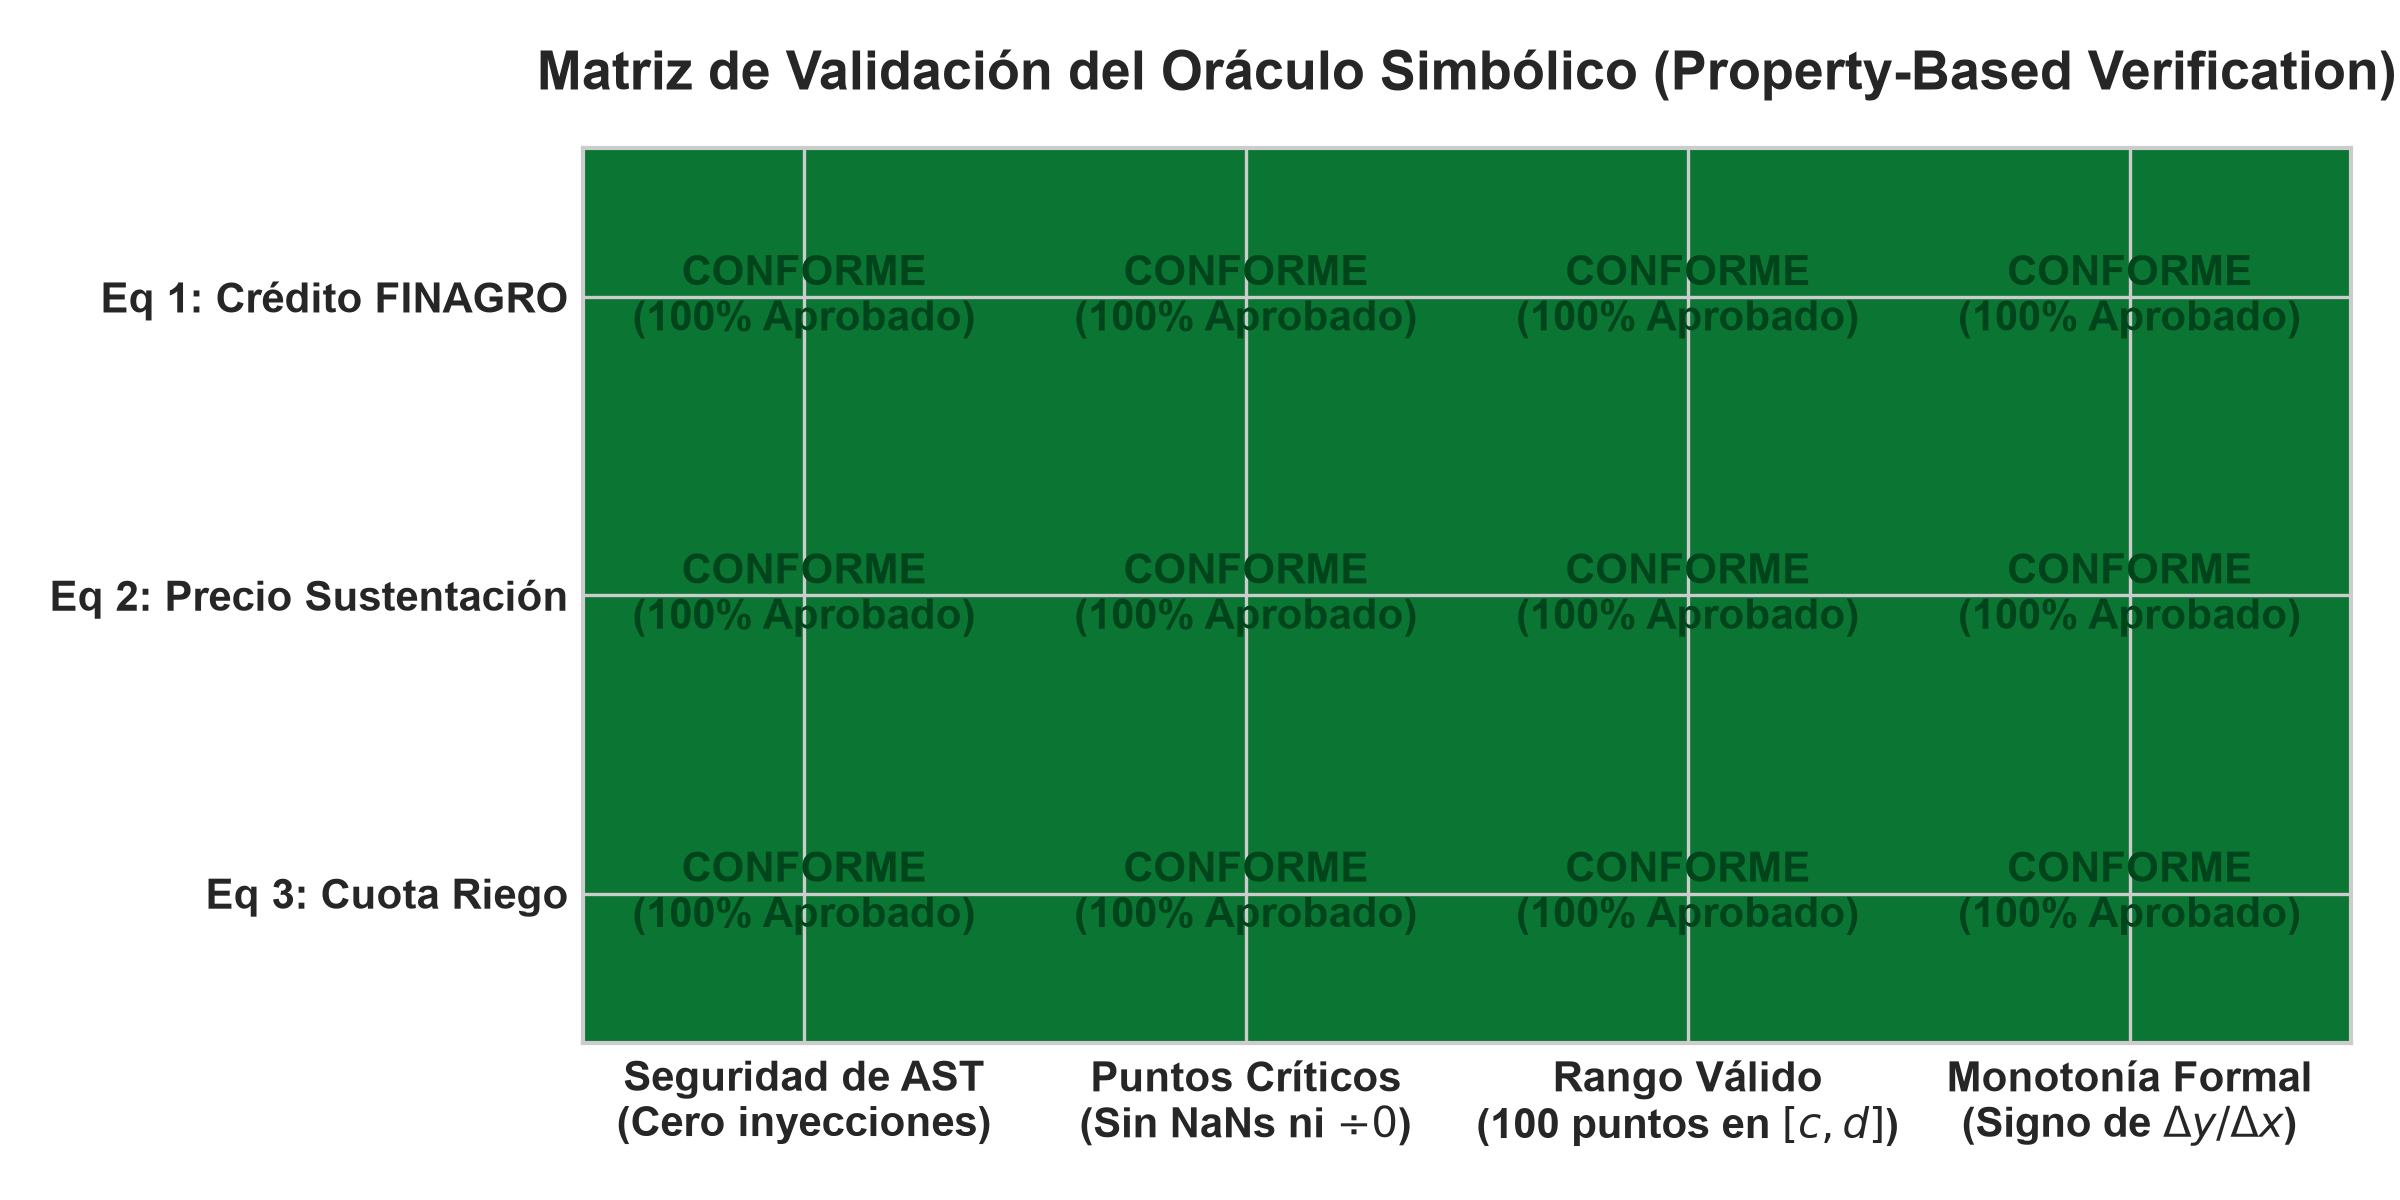
\includegraphics[width=0.88\textwidth]{../diagrams/out/fig_evaluacion_matriz_verificacion.png}
    \caption{Formal verification matrix of the symbolic oracle across synthesized institutional equations.}
    \label{fig:oracle_matrix}
\end{figure}

\begin{enumerate}[leftmargin=*]
    \item \textbf{Layer 1: Verbatim Textual Grounding (\textit{Verbatim Grounding}):}
    Every synthesized equation must include an \texttt{evidence\_verbatim\_quote} attribute. A deterministic validator (\texttt{verify\_verbatim\_quote}) conducts an exact, character-by-character substring search against the SHA-256 sealed source document. If the LLM hallucinates or alters a single word of the citation, the equation is \textbf{immediately rejected with a veracity error} (\texttt{HallucinationError}, with a strict 0.0\% tolerance threshold).

    \item \textbf{Layer 2: Parameter Anchoring to Authoritative Empirical and Legal Baselines:}
    No numerical constant is invented:
    \begin{itemize}
        \item Base interest rate $r_{\text{base}} = 0.12$ (12.0\% APR) directly reflects preferential agrarian credit lines from FINAGRO and Banco Agrario de Colombia for smallholders.
        \item Base price $P_{\text{base}} = 2,500$ COP/kg is calibrated against official SIPSA / DANE agricultural market price series for cassava and yam in Montes de Mar\'ia.
        \item Critical reserve threshold $\theta = 0.30$ complies with irrigation district operational guidelines and ecological streamflow protections (Allen et al., 1998).
    \end{itemize}

    \item \textbf{Layer 3: Deterministic Symbolic Oracle and Property-Based Testing (\texttt{SymbolicEquationVerifier}):}
    \begin{itemize}
        \item \textit{AST Security Inspection:} Parses the abstract syntax tree (\texttt{ast.parse}), restricting nodes to safe arithmetic operations (\texttt{Add}, \texttt{Sub}, \texttt{Mult}, \texttt{Div}, \texttt{Pow}, \texttt{USub}) and approved pure mathematical functions (\texttt{exp}, \texttt{log}, \texttt{sqrt}, \texttt{sin}, \texttt{cos}, \texttt{min}, \texttt{max}, \texttt{abs}). Any attribute lookup (\texttt{\_\_class\_\_}), function call, or import raises a security violation.
        \item \textit{Singularity and Critical Point Test:} Evaluates $\epsilon = 10^{-6}$ neighborhoods around denominator roots and boundary coordinates, rejecting zero-divisions, imaginary numbers, or indeterminate values (\texttt{NaN} / $\infty$).
        \item \textit{Range Confinement Test:} Uniformly samples $N=100$ points across $[x_{\min}, x_{\max}]$. The equation passes if and only if $\forall x \in [x_{\min}, x_{\max}], \, f(x) \in [y_{\min}, y_{\max}]$.
        \item \textit{Analytical Monotonicity Test:} Evaluates finite difference gradients $\Delta f / \Delta x$ across all intervals to enforce physical compliance with the declared economic incentive direction.
    \end{itemize}

    \item \textbf{Layer 4: Human-in-the-Loop Sovereign Curation Gate:}
    No verified equation enters production simulation automatically. The researcher inspects the verbatim quote, manipulates sensitivity sliders in the user interface, and certifies deployment, generating a SHA-256 stamped record in \texttt{bundle\_manifest.json}.
\end{enumerate}

% ==============================================================================
% 4. CASE STUDY: THREE SYNTHESIZED INSTITUTIONAL EQUATIONS
% ==============================================================================
\section{Empirical case study: rigorous analysis of synthesized equations}

Drawing upon authoritative documents from the 15 PDET municipalities of Montes de Mar\'ia (PATR Montes de Mar\'ia ART 2019, Law 2046 of 2020 on Local Food Procurement, and regional irrigation regulations), three functional equations were synthesized and verified:

% ------------------------------------------------------------------------------
% 4.1 EQUATION 1
% ------------------------------------------------------------------------------
\subsection{Equation 1: Credit interest rate modulated by peasant social capital}

\paragraph{Regulatory Origin:} PATR Montes de Mar\'ia (Pillar 3: Economic Reactivation and Agrarian Production, ART 2019) and FINAGRO associational credit lines.

\paragraph{Mathematical Formulation:}
\begin{equation}
    r(S_{\text{social}}) = r_{\text{base}} \cdot \Big[1 - \delta \cdot S_{\text{social}}\Big]
\end{equation}

\paragraph{Nomenclature and Variable Definitions:}
\begin{itemize}[leftmargin=*]
    \item $r$: Effective annual interest rate charged to the smallholder peasant (\% APR).
    \item $r_{\text{base}} = 0.12$: Standard baseline market lending rate (12.0\% APR) set in \texttt{BankOffice}.
    \item $\delta = 0.35$: Maximum institutional discount coefficient for community association (35\% rate subsidy).
    \item $S_{\text{social}} \in [0.0, 1.0]$: Social capital index in \texttt{PeasantFamilyBelieves} (reflecting attendance at community assemblies, communal work sessions, and local JAC boards).
\end{itemize}

\paragraph{Agronomic Interpretation:} \textit{``The annual credit interest rate decreases monotonically and linearly from 12.0\% down to 7.8\% as the smallholder expands integration into verified community associative networks''.}

\paragraph{Affected Entity and Agent Guard in EthosTerra:} Modulates loan liability inside \texttt{FromBankOfficeGuard} and the liquidity precondition for \texttt{PayDebtsGoal}.

\paragraph{Agronomic Impact:} Mitigates insolvency risks, prevents emotional distress cascades within peasant households, and preserves operating liquidity for agricultural inputs and seed acquisition.

\begin{figure}[H]
    \centering
    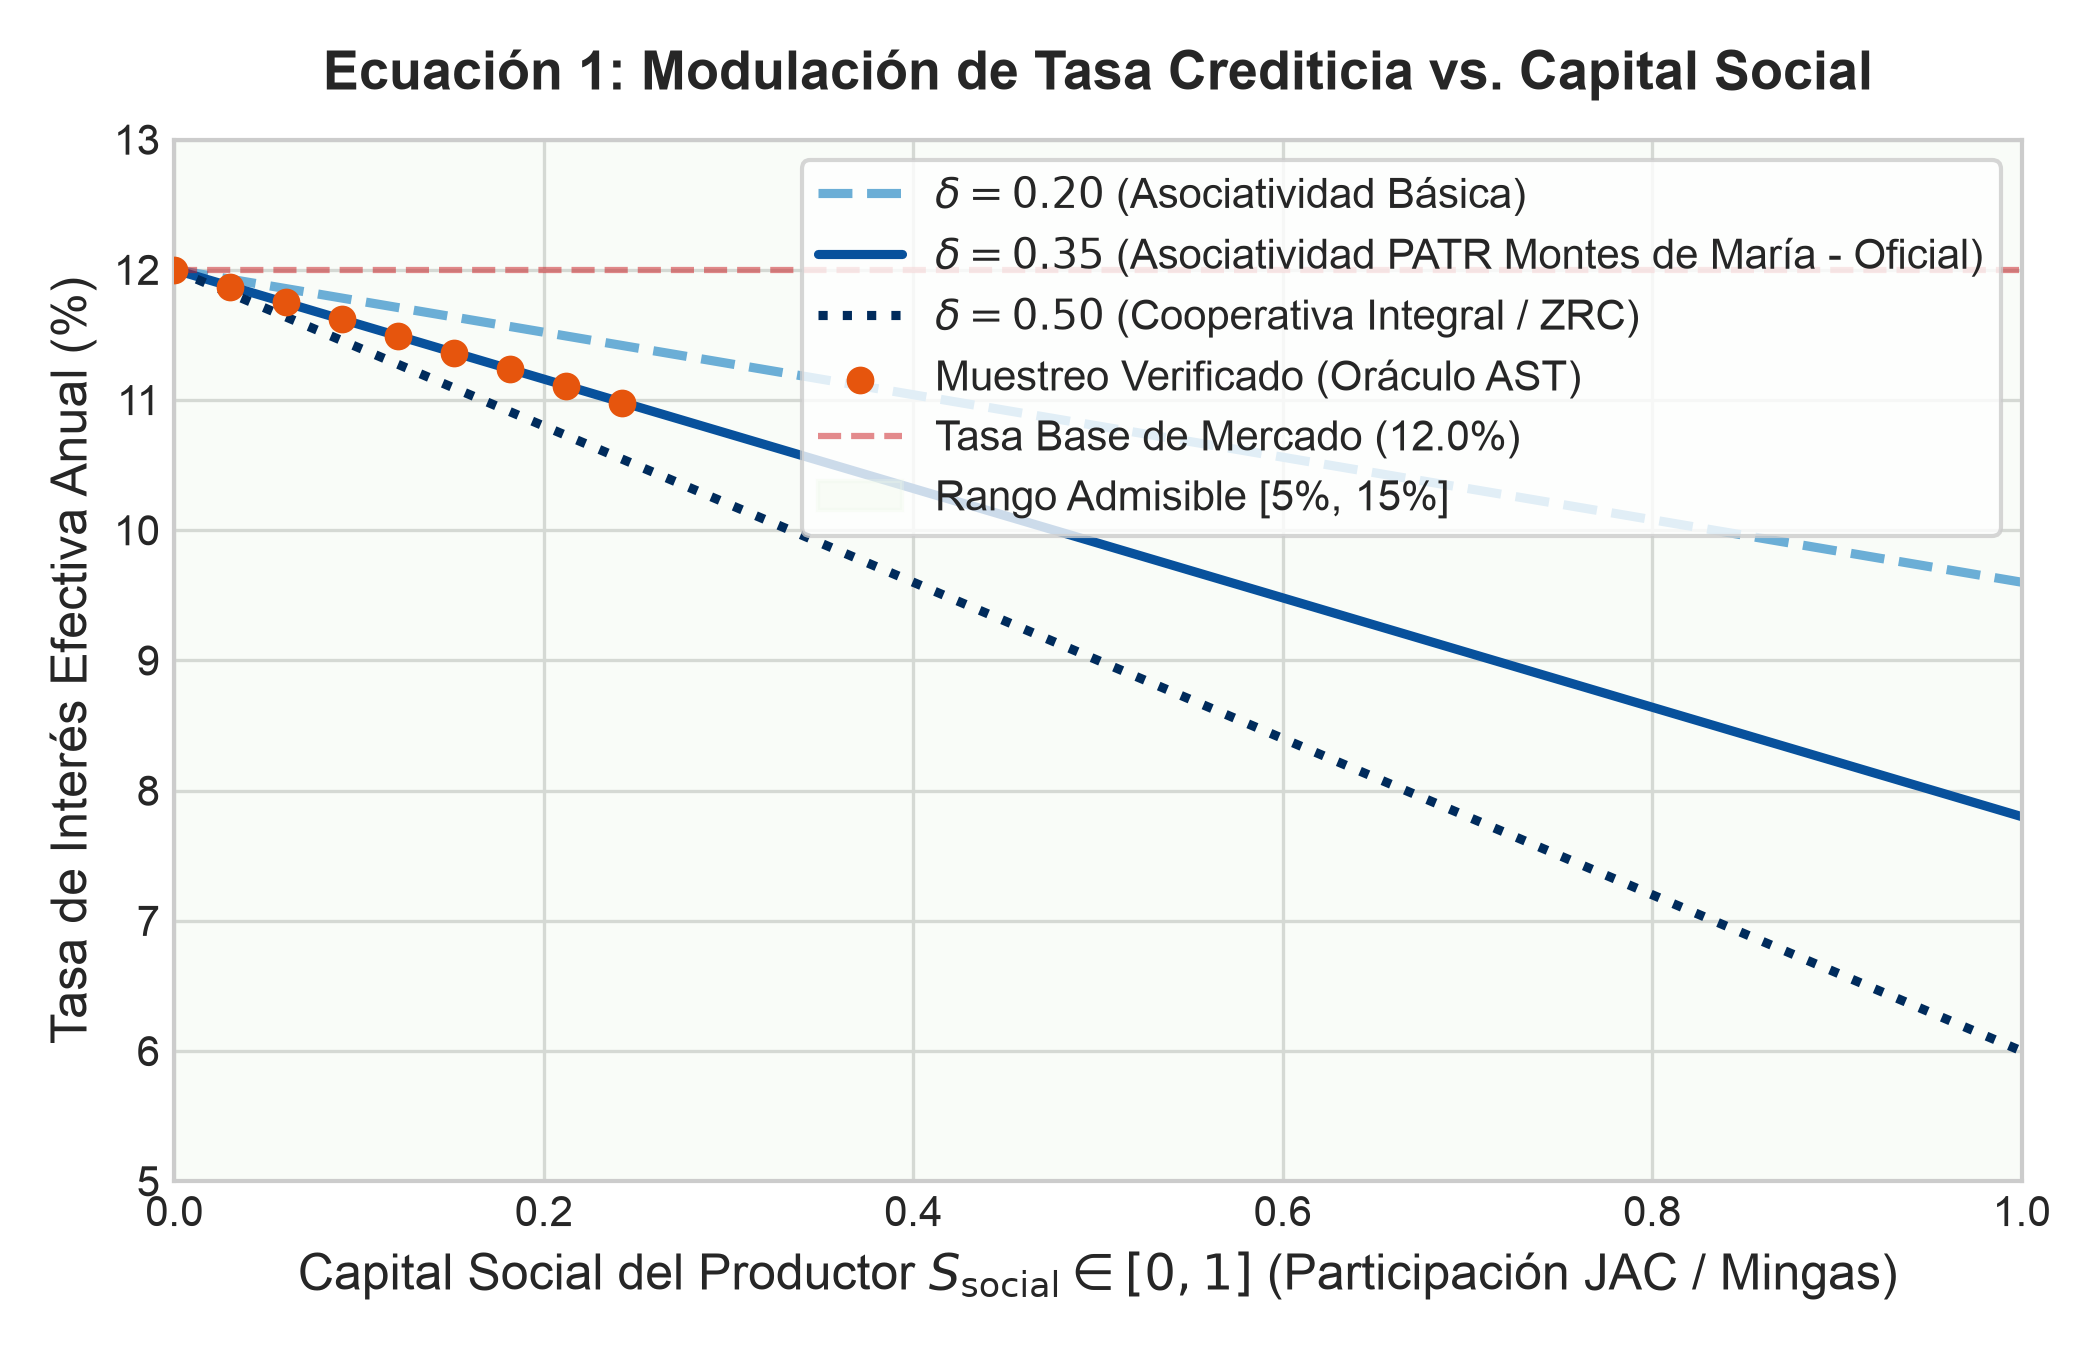
\includegraphics[width=0.78\textwidth]{../diagrams/out/fig_eq1_credito_capital_social.png}
    \caption{Effective credit interest rate curve as a function of peasant social capital, showing $\delta$ sensitivity bands and AST oracle verification samples.}
    \label{fig:eq1_en}
\end{figure}

% ------------------------------------------------------------------------------
% 4.2 EQUATION 2
% ------------------------------------------------------------------------------
\subsection{Equation 2: Local support price response to crop yield shock}

\paragraph{Regulatory Origin:} Law 2046 of 2020 on Public Procurement of Local Food (Congress of Colombia, 2020).

\paragraph{Mathematical Formulation:}
\begin{equation}
    P_{\text{mkt}}(Y_{\text{rel}}) = P_{\text{base}} \cdot \Big[1 + \alpha \cdot \exp\left(-\beta \cdot Y_{\text{rel}}\right)\Big]
\end{equation}

\paragraph{Nomenclature and Variable Definitions:}
\begin{itemize}[leftmargin=*]
    \item $P_{\text{mkt}}$: Guaranteed institutional purchase price per kilogram delivered (\$ COP / kg).
    \item $P_{\text{base}} = 2,500$: Standard commercial support price in \texttt{MarketPlace} (\$2,500 COP/kg for cassava/yam).
    \item $\alpha = 0.40$: Maximum institutional protection coefficient under production collapse (+40\% price premium).
    \item $\beta = 2.50$: Exponential decay rate governing agrarian shock damping.
    \item $Y_{\text{rel}} \in [0.0, 1.0]$: Relative crop yield ($\text{realized biomass} / \text{expected biomass}$).
\end{itemize}

\paragraph{Agronomic Interpretation:} \textit{``The guaranteed purchase price rises in a convex, monotonically decreasing curve when crop yields plunge due to drought or pests, ensuring that small marketable surpluses sustain basic household survival thresholds''.}

\paragraph{Affected Entity and Agent Guard in EthosTerra:} Modulates the unit purchase price in \texttt{FromMarketPlaceGuard} and the cash flow trajectory of \texttt{SellCropGoal}.

\paragraph{Agronomic Impact:} Shields smallholders against devastating market volatility following extreme weather disruptions (e.g., ENSO El Ni\~no droughts), stabilizing rural family livelihood.

\begin{figure}[H]
    \centering
    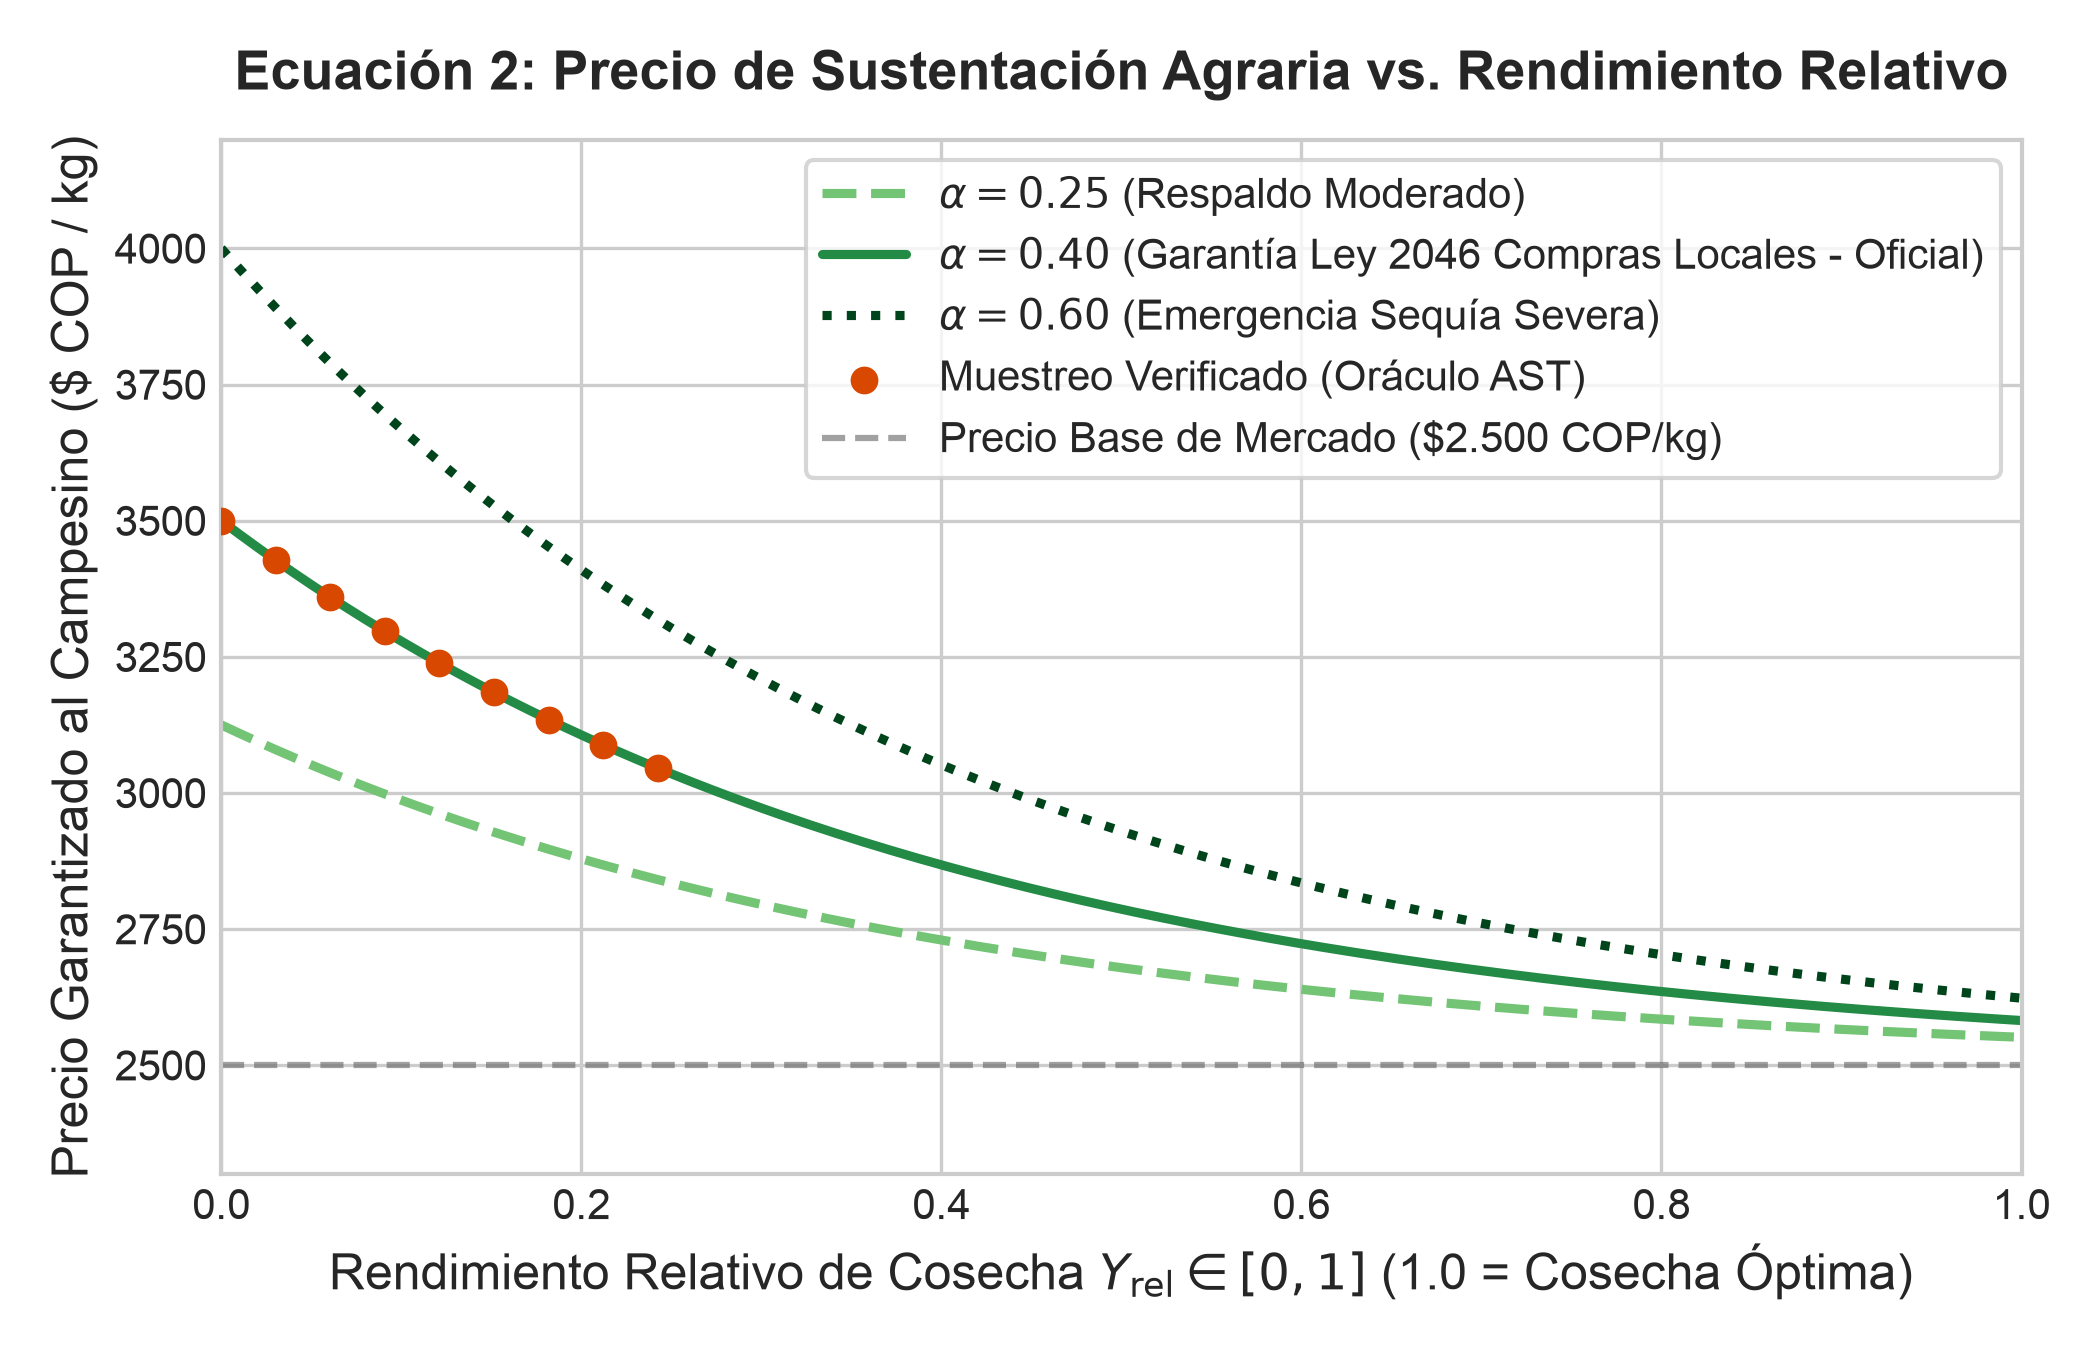
\includegraphics[width=0.78\textwidth]{../diagrams/out/fig_eq2_precio_sustentacion_cosecha.png}
    \caption{Agrarian support price curve under relative harvest yield shocks, with $\alpha$ sensitivity bands and property-based verification sample points.}
    \label{fig:eq2_en}
\end{figure}

% ------------------------------------------------------------------------------
% 4.3 EQUATION 3
% ------------------------------------------------------------------------------
\subsection{Equation 3: Irrigation district water quota based on reservoir level}

\paragraph{Regulatory Origin:} Operational regulations of small-scale irrigation districts in Mar\'ia La Baja and FAO-56 irrigation standards (Allen et al., 1998; Ostrom, 1990).

\paragraph{Mathematical Formulation:}
\begin{equation}
    Q_{\text{water}}(w) = Q_{\text{max}} \cdot \left[\frac{w^2}{w^2 + \theta^2}\right]
\end{equation}

\paragraph{Nomenclature and Variable Definitions:}
\begin{itemize}[leftmargin=*]
    \item $Q_{\text{water}}$: Daily water allocation delivered to peasant parcel (Liters / ha / day).
    \item $Q_{\text{max}} = 100.0$: Maximum capacity discharge under full infrastructure availability.
    \item $\theta = 0.30$: Critical ecological streamflow threshold (30\% reservoir storage capacity).
    \item $w \in [0.0, 1.0]$: Relative reservoir storage level in cellular automaton \texttt{AgroEcosystem}.
\end{itemize}

\paragraph{Agronomic Interpretation:} \textit{``Water delivery follows a smooth Hill sigmoidal transition: it drops steeply toward zero once reservoir storage drops below the 30\% critical reserve threshold, and saturates asymptotically toward 100 L/ha/day under full capacity conditions''.}

\paragraph{Affected Entity and Agent Guard in EthosTerra:} Directly dictates \texttt{water\_available} inside \texttt{PeasantFamilyBelieves} and the execution feasibility of \texttt{IrrigateCropsGoal}.

\paragraph{Agronomic Impact:} Captures community-governed water management rules (Ostrom, 1990), prompting peasant agents to trigger soil moisture conservation practices whenever $w < \theta$.

\begin{figure}[H]
    \centering
    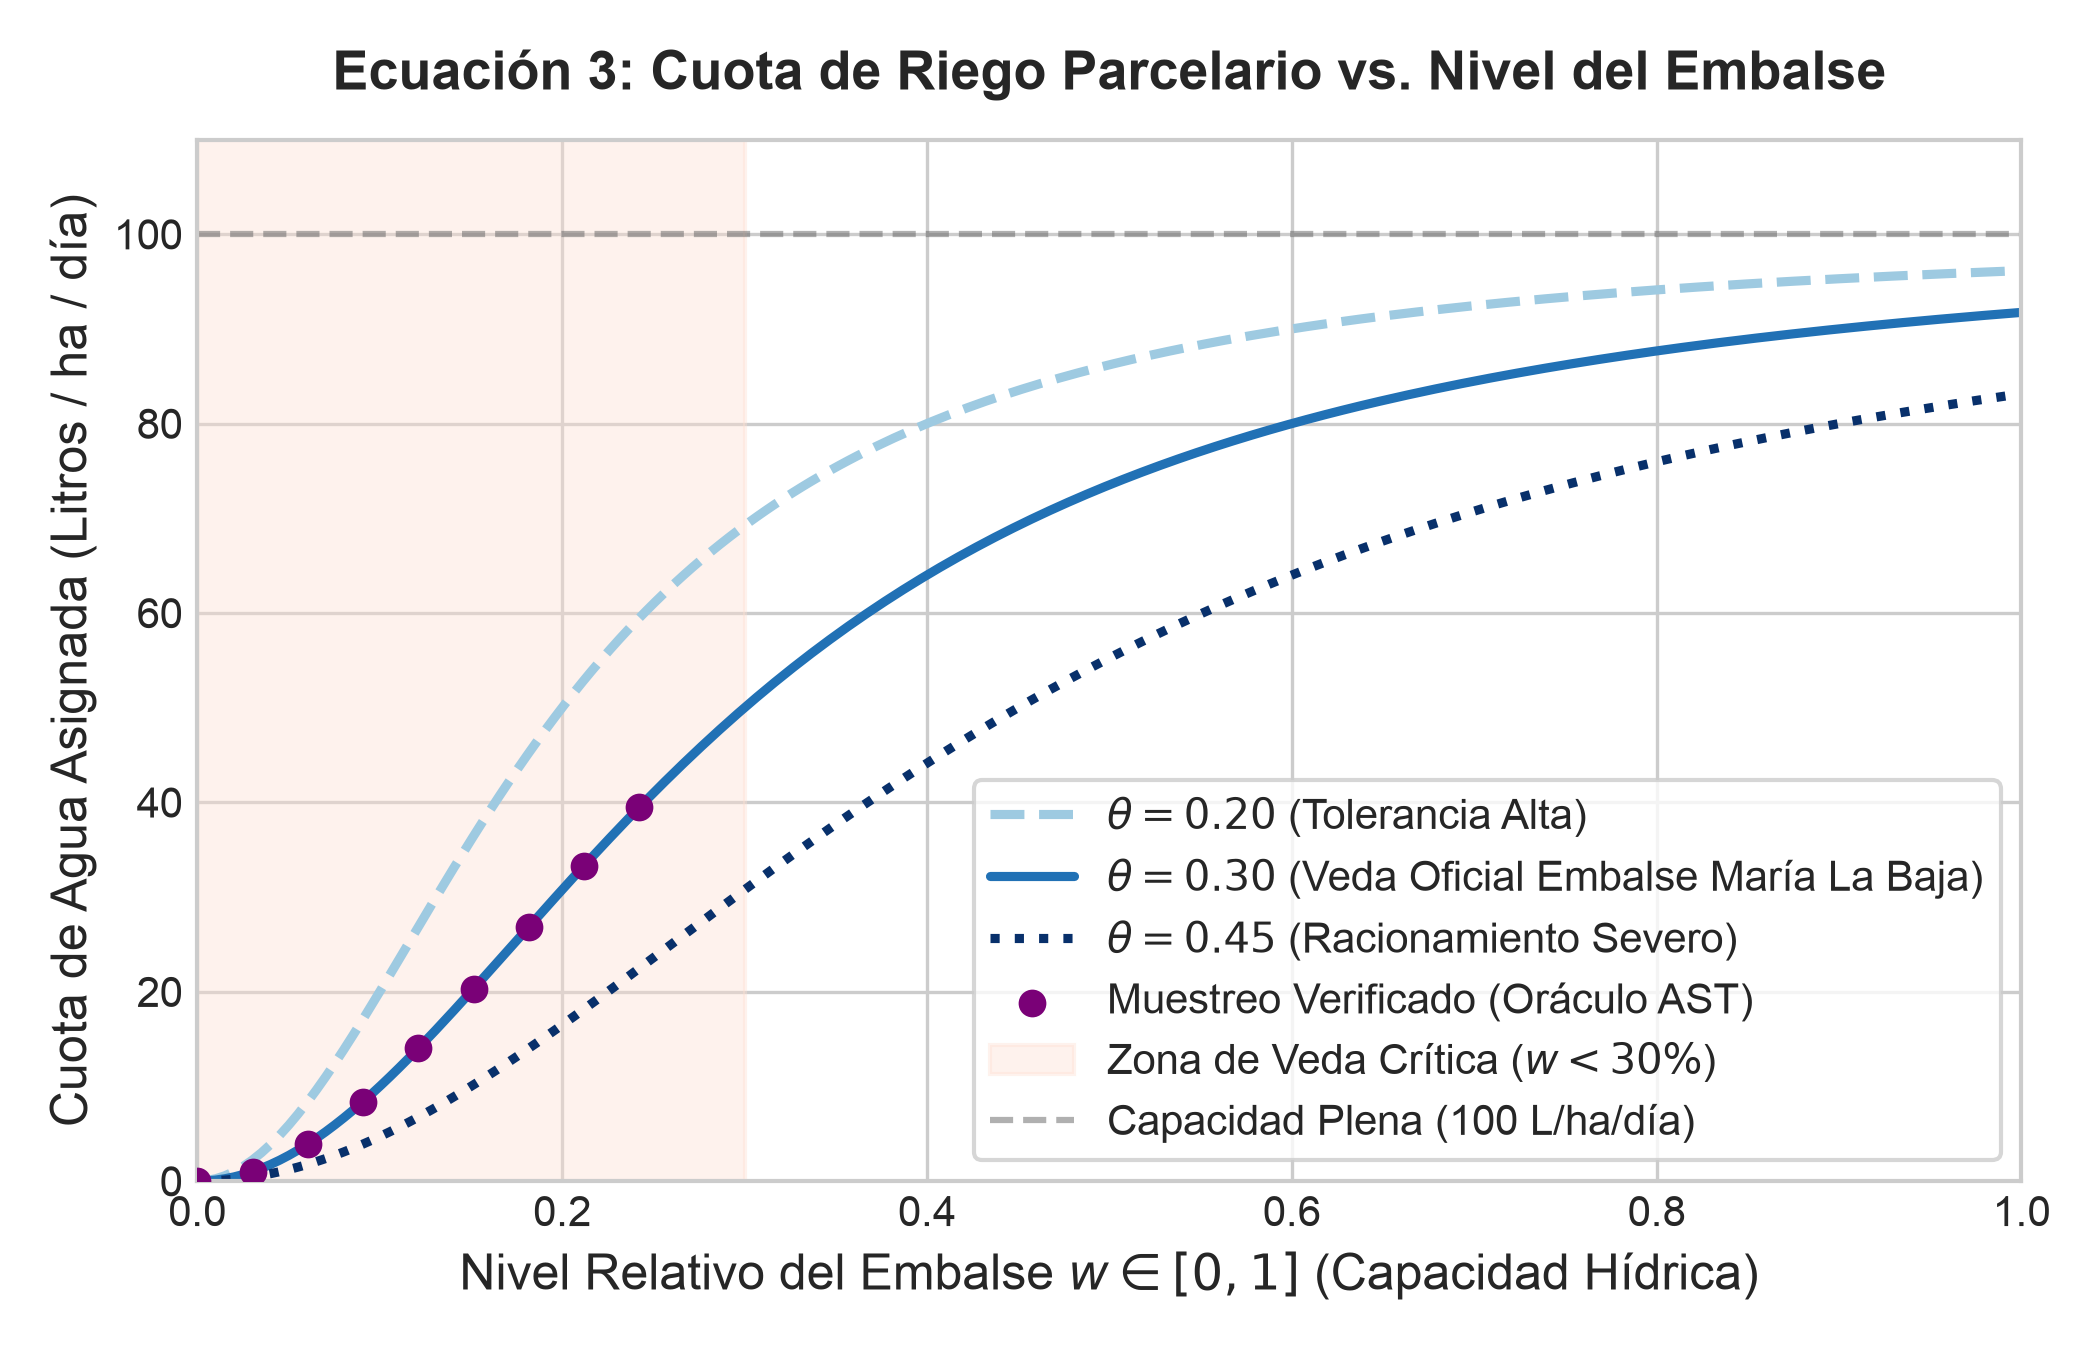
\includegraphics[width=0.78\textwidth]{../diagrams/out/fig_eq3_cuota_riego_reserva.png}
    \caption{Daily irrigation delivery curve as a function of relative reservoir volume, delineating critical drought curtailment ($w < 30\%$) and supply saturation.}
    \label{fig:eq3_en}
\end{figure}

% ==============================================================================
% 5. USER INTERFACE INTEGRATION (ATLAS UI)
% ==============================================================================
\section{User interface integration: interactive curation console}

To streamline verification and oversight by research advisors and domain specialists, the agronomic tab of \texttt{AtlasView.tsx} in the React / TypeScript frontend was substantially enhanced:

\begin{itemize}[leftmargin=*]
    \item \textbf{Symbolic Equations Console:} Introduces a dedicated panel titled \textit{``Laboratorio de Ecuaciones Simb\'olicas Institucionales (Semana 11 - B7)''}, featuring interactive navigation buttons to toggle between all three verified formulas (\textit{Eq 1: FINAGRO Credit}, \textit{Eq 2: Support Price}, \textit{Eq 3: Irrigation Quota}).
    \item \textbf{Real-Time Sensitivity Sliders:} Enables researchers to manipulate continuous input sliders ($S_{\text{social}}$, $Y_{\text{rel}}$, $w$) and observe immediate computational outputs alongside detailed agronomic context.
    \item \textbf{Dynamic Formal Audit Badges:} Four live audit badges verify the core mathematical invariants of the deterministic oracle: \textit{Monotonicity Conformance}, \textit{Bounded Range}, \textit{Zero Singularities}, and \textit{AST Security Approval}.
    \item \textbf{Ontological Traceability:} Each equation explicitly exhibits its institutional stratum badge (\texttt{institutional\_policy}) and target entity within EthosTerra (\texttt{BankOffice}, \texttt{MarketPlace}, \texttt{AgroEcosystem}).
\end{itemize}

% ==============================================================================
% 6. DECOUPLED ADAPTER ARCHITECTURE
% ==============================================================================
\section{Decoupled simulation adapter architecture}

The \texttt{EthosTerraDecoupledAdapter} guarantees repository immutability and complete segregation:
\begin{itemize}[leftmargin=*]
    \item Writes exclusively to the isolated sandbox directory \texttt{outputs/simulation\_sandbox/}, ensuring zero modifications to the \texttt{EthosTerra} repository tree.
    \item Generates \texttt{world\_modifiers.json}, consolidating macro-institutional directives targeting bank, market, and environmental entities.
    \item Emits \texttt{bundle\_manifest.json}, certifying the SHA-256 hash of each compiled specification alongside curator metadata and UTC timestamps.
\end{itemize}

% ==============================================================================
% 7. EMPIRICAL TEST SUITE RESULTS
% ==============================================================================
\section{Empirical evidence and automated test results}

The project's test suite was expanded to 278 passing test cases under \texttt{make test-unit}:

\begin{table}[H]
\centering
\small
\caption{Quantitative results across automated unit test suites.}
\label{tab:tests}
\begin{tabularx}{\textwidth}{lp{6.0cm}rX}
\toprule
\textbf{Test Module} & \textbf{Evaluated Scope} & \textbf{Cases} & \textbf{Status} \\
\midrule
\texttt{test\_symbolic\_equation\_verifier.py} & AST security, injection, monotonicity, singularities & 13 & 100\% Passed \\
\texttt{test\_institutional\_schemas\_*.py} & Pydantic V2, institutional tiers, YAML compilation & 6 & 100\% Passed \\
\texttt{test\_ethosterra\_decoupled\_adapter.py} & Sandbox bundles, world\_modifiers, API endpoints & 5 & 100\% Passed \\
Legacy Suites Weeks 5--10 & DMR canary, Pure Case, Conflict Case, CRUD, Auth & 254 & 100\% Passed \\
\midrule
\textbf{Overall Total} & \textbf{Monorepo integral test coverage} & \textbf{278} & \textbf{278/278 (100\%)} \\
\bottomrule
\end{tabularx}
\end{table}

Furthermore, the React / TypeScript frontend built cleanly in 350\,ms without type errors:
\begin{lstlisting}[language=bash, caption={Clean frontend build output.}]
> frontend@0.0.0 build
> tsc -b && vite build

dist/index.html                                  0.47 kB | gzip:   0.30 kB
dist/assets/maplibre-gl-worker-VaXr2Fck.mjs    508.31 kB
dist/assets/index-DAotwnwW.css                 158.46 kB | gzip:  24.17 kB
dist/assets/index-CLOgv-g6.js                1,748.94 kB | gzip: 466.00 kB
built in 350ms (zero TypeScript errors)
\end{lstlisting}

% ==============================================================================
% 8. REPRODUCIBILITY INSTRUCTIONS
% ==============================================================================
\section{Technical reproduction commands}

\begin{lstlisting}[language=bash, caption={Step-by-step local validation commands.}]
# 1. Run all 278 automated unit tests
make test-unit

# 2. Re-generate publication figures
uv run --with matplotlib --with numpy --with pydantic python scripts/generate_scientific_plots.py

# 3. Build frontend bundle
pnpm --dir apps/ui build
\end{lstlisting}

% ==============================================================================
% 9. AUTHORITATIVE REFERENCES
% ==============================================================================
\section{References}
\begin{enumerate}[leftmargin=*]
    \item Agencia de Renovaci\'on del Territorio (ART). (2019). \textit{Plan de Acci\'on para la Transformaci\'on Regional (PATR) -- Subregi\'on Montes de Mar\'ia}. Presidencia de la Rep\'ublica de Colombia, Bogot\'a D.C.
    \item Allen, R. G., Pereira, L. S., Raes, D., \& Smith, M. (1998). \textit{Crop evapotranspiration: Guidelines for computing crop water requirements}. FAO Irrigation and Drainage Paper No. 56, Food and Agriculture Organization of the United Nations, Rome.
    \item Bratman, M. E. (1987). \textit{Intentions, Plans, and Practical Reason}. Harvard University Press, Cambridge, MA.
    \item Congreso de la Rep\'ublica de Colombia. (2020). \textit{Ley 2046 de 2020: Por la cual se establecen mecanismos para promover la participaci\'on de peque\~nos productores locales agropecuarios en los mercados de compras p\'ublicas de alimentos}. Diario Oficial No. 51.417, Bogot\'a D.C.
    \item Departamento Administrativo Nacional de Estad\'istica (DANE). (2024). \textit{Marco Geoestad\'istico Nacional (MGN) y Codificaci\'on DIVIPOLA}. DANE, Bogot\'a D.C.
    \item Ortony, A., Clore, G. L., \& Collins, A. (1988). \textit{The Cognitive Structure of Emotions}. Cambridge University Press, Cambridge.
    \item Ostrom, E. (1990). \textit{Governing the Commons: The Evolution of Institutions for Collective Action}. Cambridge University Press, Cambridge.
    \item Rao, A. S., \& Georgeff, M. P. (1995). \textit{BDI agents: from theory to practice}. In Proceedings of the First International Conference on Multi-Agent Systems (ICMAS-95), pp. 312--319.
\end{enumerate}

\end{document}
